\documentclass[a4paper]{article}
\usepackage{amsmath}
\usepackage{graphicx}
\usepackage[utf8]{inputenc}
\usepackage[T1]{fontenc}
\usepackage[french]{babel}
\usepackage{amsfonts,amsmath,amssymb}
\usepackage{float}
\usepackage{graphicx}
\usepackage{amsmath}
\usepackage{newunicodechar}


\title{\textbf{Rapport d'alternance Master 2 Ingénierie logicielle\\ }}
\author{\textbf{MOUTARAJJI} Mouhyi-Eddine\
\\Encadré par :\\\textbf{SALAÜN} Gaël \\\textbf{BOURDÉ} Annabel }
\begin{document}
\date{}

\begin{figure}
\centering

\includegraphics[width=1.1\textwidth]{diagrammes/logoisticfr_0.png}
\end{figure}


\maketitle

\newpage

\tableofcontents
~
\newpage



\section{Contexte général}
\subsection{Rectorat de l’académie de Rennes}

Le rectorat de l'académie de Rennes est une circonscription administrative propre à
l’Éducation Nationale.\\
Elle regroupe 4 directions des services départementaux de l'Éducation Nationale : 
Côtes d'Armor, Finistère, Ille-et-Vilaine et Morbihan. Chaque direction des services départementaux de l'éducation nationale est placée sous la responsabilité d'un inspecteur d'académie, directeur académique des services de l'Éducation nationale.Son rôle au sein de ces départements est de gérer les personnels, les élèves, les moyens financiers, les examens... de tous les établissements scolaires, depuis la maternelle jusqu'au lycée.

\subsection{Organisation}

\subsection{Architecture des projets}

Au sein du rectorat Rennes, la majorité de l'équipe d'informatique  développent des applications web. Il existe plusieurs types d'application (métiers,outils...). Ces applications sont constituées de deux modules, Back-end \&  Front-end.

\subsubsection{Back-end}

Le Back-End, c’est la partie du code qui est exécutée par le serveur, il s’agît d'un serveur fournissant une API gérant la persistance des données et la logique de l'application.La majorité des applications du rectorat sont développées en framework Spring-boot et en langage Java et il existe quelques applications développées en langage Kotlin dont l'application Apptour.

L'architecture des projets du rectorat est unique dans tous les projets afin  de faciliter la prise en main de ces derniers et avoir le même point de vue au sein du l'équipe.

Le back-end des applications se décomposent de plusieurs couches: 

une couche Repository/DAO: Repositories sont des interfaces héritant de l'interface Repository. L'objectif de ces interfaces consiste à rendre la création de la couche d'accès aux données (requêtes SELECT, UPDATE...) plus rapide.

une couche Service: Elle permet de séparer les opérations effectuées par le contrôleur et celles qui concernent le modèle des données. Toute action devrait passer par cette couche.

Une couche Contrôller: Il s'agit de l'Api qui permet de répondre à toutes les requêtes envoyées par le client. 

\begin{figure}[H]
	\centering
 		\fbox{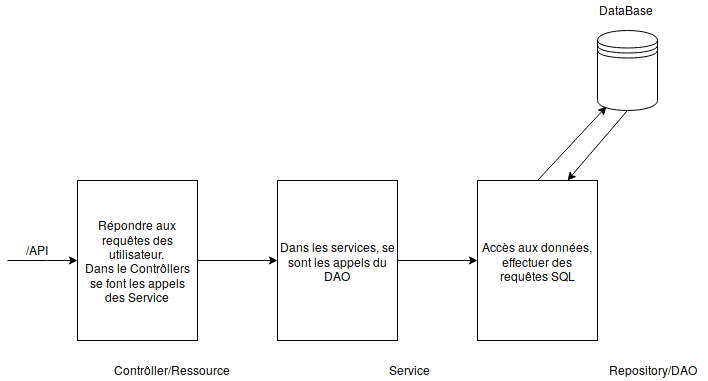
\includegraphics[width=1.2\textwidth]{diagrammes/ArchitectureProjet.png}} 
  		\caption{Arichtecture Back-end d'une application web}
	\end{figure}

\subsubsection{Front-end}
Le Front-end est la partie visible par les utilisateurs des applications web. Elle comprend l'interface graphique par laquelle nos utilisateurs vont interagir avec 
le reste du système (Back-end).


Le Front-end des applications web du rectorats sont développées en plusieurs langages. La plupart de ces applications  sont codées avec le triplet HTML,CSS \& JavaScript. Tandis que ces derniers mois, l'équipe informatique commence à intégrer le langage React.js  afin de monter en compétences et découvrir des nouveaux langages plus récents. 

\textbf{HTML:} HTML est une technologie et un standard qui permet d'afficher le contenu d'une application sur le web. Le langage reprend la syntaxe de XML,c'est-à-dire, une imbrication de balise/élément/tag les uns dans les autres.

\textbf{CSS:} CSS, est une technologie complémentaire à HTML, c'est elle qui va permettre d'ajouter des couleurs, des ombres, de mettre en forme le texte, de positionner les blocs, etc. Elle sert à mettre en forme une page web. 

\textbf{JavaScript:} JavaScript, au contraire de HTML et CSS, n'est pas un langage de présentation mais de programmation, qui plus est, objet orienté prototype. Il permet de rendre plus dynamique une application web grâce à la manipulation de l'API DOM (Document Object Model) et de l'AJAX (Asynchronous JavaScript And XML).

\textbf{React:} Le défaut de JavaScript, mais qui est aussi sa force, est sa grande flexibilité (typage dynamique, première ordre, point virgule optionnel...). On peut donc arriver très facilement à un code illisible et non maintenable. Le framework React apporte beaucoup de solutions à ces problèmes, avec sa façon de manipuler la DOM (via un moteur de template), l'utilisation de TypeScript (une amélioration du JavaScript par Microsoft.De plus, il est très facile de générer un environnement React pour un projet. C'est pour ces raisons que l'équipe informatique du rectorat commence à prendre en main ce Langage et l’intégrer dans les nouveaux projets et les nouvelles applications web. 

\begin{figure}[H]
	\centering
 		\fbox{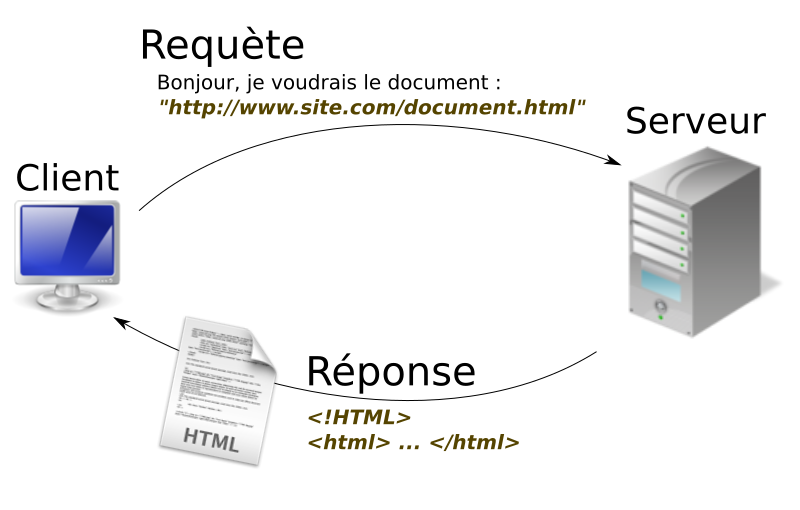
\includegraphics[width=1.2\textwidth]{diagrammes/schema-serveur.png}} 
  		\caption{Application Web classique}
	\end{figure}

\subsection{Méthodes de travail}
\subsubsection{Méthodologie agile}

Les équipes informatiques du rectorat fonctionnent en méthodologie agile, chaque équipe effectue un Daily afin que chaque personne puisse présenter sur quoi elle a travaillé la veille et sur quoi elle compte continuer le jour même. Dans mon cas, j'étais le seul développeur dans mon projet, je faisais un Daily tout les jours avec mes maîtres d'alternances pour que je puisse dire sur quoi je travaillais et leurs poser des questions en cas de blocages. 

\subsubsection{Communication}

Pour communiquer, l'équipe informatique utilise l'outil de messagerie instantané RocketChat. Il permet de créer différents
channels pour chaque équipe, des channels de veille ont été également crées pour de la veille technologies.

Nous utilisons aussi l'outil Calendar (un outil développer par Oracl) qui permet d’organiser les réunions.  

\subsubsection{Dockerisation}

Le logiciel Docker permet de créer, déployer et exécuter des conteneurs de manière efficace. Un conteneur enveloppe l’application d’un logiciel dans une boîte invisible avec tout ce dont il a besoin pour s’exécuter. Cela comprend le
système d’exploitation, le code de l’application, le runtime, les outils système et les librairies. Les conteneurs Docker sont construits à partir des images Docker.

Ils sont légers, portables et permettent aux développeurs de créer, déployer et exécuter efficacement des applications distribuées. En outre, ils permettent à une application d’être empaquetée et déplacée facilement, augmentant ainsi la simplicité d’une infrastructure.

\subsubsection{Versionning}

L'équipe informatique utilise Git sur la plateforme Gitlab hébergé par la Forge comme gestionnaire de version. 


\section{Objectifs et missions de l'alternance}

\subsection{Objectif du projet}

Au sein du rectorat, le pôle DINAMO se charge de réaliser les applications web métiers et autres. L'équipe informatique utilise différentes façons pour documenter leur applications. La plupart du temps elle utilise une documentation écrite (Manuel Utilisateur), une chose qui ne rend pas facile aux utilisateurs d’interagir avec l'application et comprendre la documentation. 


C'est pour cette raison que Monsieur JOSSO Clément,le product Owner du projet(PO), a voulu mettre en œuvre une documentation interactive dans l'application métier Solycee afin de permettre aux utilisateurs de l'application de se auto-documenter et interagir directement avec la page web. Nous avons utilisé un outil nommé BootstrapTour pour réaliser cette documentation. 

Le but final du projet est de permettre aux administrateurs d'être autonomes et de pouvoir rajouter ou modifier les tours ainsi que leurs  étapes dans leurs applications. Nous avons donc crée un web service(AppTour) où sont sauvegardé tous les tours et leurs étapes.

\subsection{Solycee}

Solycee est une application métier créée par le rectorat et destinée à la gestion des offres et demandes de stages. Elle permet aux collèges et aux lycées d'inscrire leurs élèves aux mini-stages proposés par les lycées.  

L'application serveur est réalisé en Java avec l'utilisation des composants du framework Spring.L'interface est codé avec le triplet HTML,CSS \& Javascript en intégrant du Thymeleaf pour le traitement des vues.  

\subsubsection{Aspect technique}

Le projet est implémenté selon le patron de conception MVC et réalisé avec plusieurs technologies, la plupart de ces dernières sont open-source.L'application est implémenté avec un back-end et un Front-end.

Le back-end a été implémenté avec le framework Spring et le langage Java. Le coté interface (Front-end) a été réalisé avec le moteurs de templâte Thymeleaf. 

Voici maintenant une présentation plus précises sur les principaux outils utilisés:

\textbf{Spring:}  Spring est un framework libre pour construire et définir l'infrastructure d'une application java dont il facilite le développement et les tests.

\begin{itemize}
	\item \textbf{Spring MVC} : Spring MVC est un framwork qui permet d’implémenter des applications selon le design pattern MVC. Donc, comme tous autre MVC framework, Spring MVC se base sur le principe décrit par le schéma ci-dessous :
	

\begin{figure}[H]
	\centering
 		\fbox{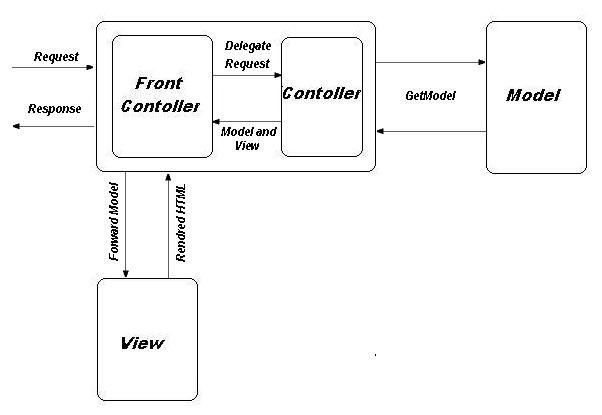
\includegraphics[width=1.2\textwidth]{diagrammes/mvc.jpg}} 
  		\caption{Schéma du patron de conception MVC}
	\end{figure}
	
	\item \textbf{Spring Security }: Spring Security est un Framework de sécurité léger qui fournit une authentification et un support d’autorisation afin de sécuriser les applications Spring.
\end{itemize} 

\textbf{Maven:} Maven est un outil de construction de projets (build) open source développé par la fondation Apache, initialement pour les besoins du projet Jakarta Turbine. Il permet de faciliter et d'automatiser certaines tâches de la gestion d'un projet Java.

\textbf{Thymeleaf:} Thymeleaf est un  Java XML/XHTML/HTML5 Template Engine qui peut travailler à la fois dans des environnements Web (Servlet) et celui de non Web. Il est mieux adapté pour diffuser XHTML/HTML5 sur View (View Layer) des applications Web basées sur MVC. Mais il peut traiter n'importe quel fichier XML même dans les environnements hors ligne. Il fournit une intégration complète de Spring Framework. 

\subsubsection{Travail réalisé}

Dans le projet Solycee, j'ai principalement travaillé sur la partie Front-end. j'ai réalisé plusieurs tâches soit en rajoutant des nouvelles vue et des nouveaux composants dans les pages web et/ou en rajoutant des nouvelles fonctionnalités sur les composants existant. Voici une présentation plus précises de toutes les tâches réalisées: 
\begin{itemize}
\item Rajout d'une modal pour prévenir les utilisateurs de la  présence d'un bouton aide pour déclencher la documentation interactif.

\begin{figure}[H]
	\centering
 		\fbox{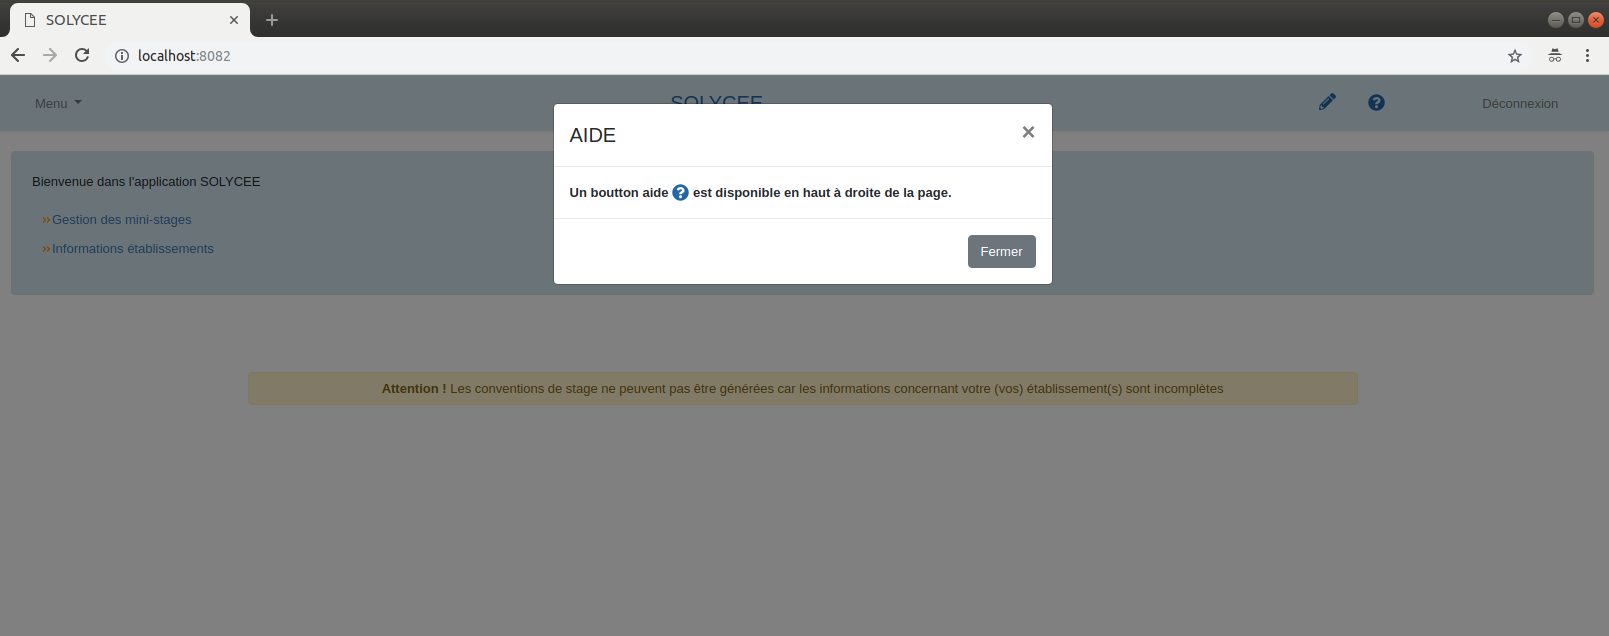
\includegraphics[width=1.2\textwidth]{diagrammes/aide_modal.png}} 
  		\caption{Image page d'accueil Solycee}
	\end{figure}
   
\item Rajout du Bootstrap Tour : Il s'agit de l'ajout d'un bouton sur toutes les pages web de l'application. En appuyant dessus ça déclenche les popup avec les tours (Element, Title \& content)  

\begin{figure}[H]
	\centering
 		\fbox{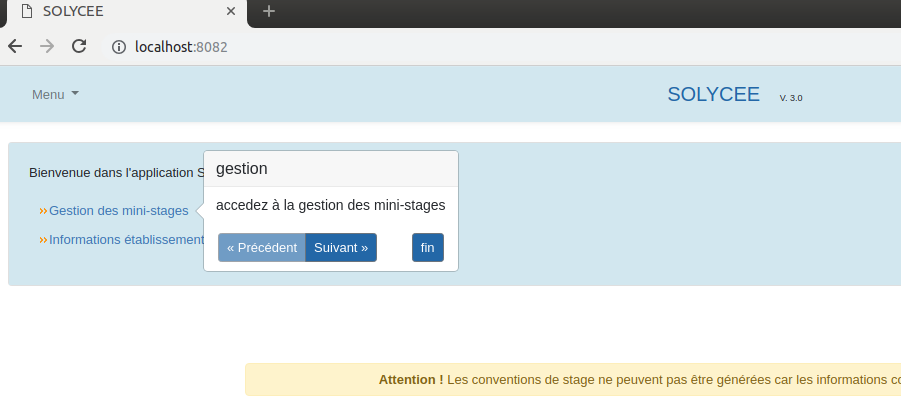
\includegraphics[width=1.2\textwidth]{diagrammes/exemple_Tour.png}} 
  		\caption{Exemple d'une étape de Bootstrap Tour}
	\end{figure}
\end{itemize} 

\subsection{AppTour}     

\subsection{Bootstrap Tour : Une visite guidée interactive}
 
Bootstrap tour est une petite librairie JavaScript permettant de présenter de façon assez simple l’application, l’avantage, comme pour toutes les librairies en fait, c’est qu’il y a déjà des bouts de fonctionnalités toutes faites, ce qui évite de réimplémenter le code. Bootstrap tour est une implémentation qui sert à créer une visite guidée pour une application. 



\end{document}
